\documentclass[authoryearcitations]{UoYCSproject}
\usepackage[dvipdfm]{graphicx}
\usepackage[dvipdfm]{color}
\usepackage{amsmath, amsthm, amssymb}
\usepackage{a4wide}
\usepackage{simpsons}
\usepackage{subfig}
\author{Jose Manuel Calderon}
\title{Modeling Quantum Dots Using Geometric Primitives}
\date{2011-September-14}
\supervisor{Prof. Samuel L. Braunstein}
\MNC
\wordcount{1337}
\abstract{ \LaTeXe\ is a document markup and processing system built
  upon Donald Knuth's type-setting system, \TeX.}
   


\begin{document} 
\maketitle
\chapter{Introduction}

\chapter{Literature Review}
In this chapter we will look at and discuss some of the literature relevant to this project. 
In order to properly understand the system being modeled we will briefly touch on quantum mechanics
and some of the necessary mathematics. In the second section we will look at numerical methods with
particular focus on the finite difference method.
We will also look at various matrix representations that are present in the tools used for our
model. 
 
\section{Quantum Dots}
Since being discovered in the 1970's by Leo Esaki and 
Raphael Tsu quantum confinement in semiconductors has been of interest to physicists and engineers for numerous applications 
\cite{dots, reed}. Having at first demonstrated quantum confinement in one dimension, it was correctly predicted that 
confinement in two and three dimensions would be feasible \cite{dots}. A structure that exhibits 
quantum confinement in three dimensions is known as a quantum dots (QD from now on). Quantum wires and 
wells correspond to confinement in one and two dimensions respectively \cite{dots}. In this section we will discuss the
background necessary to be able to model QDs. This will include a brief look at some of the underlying physics with an 
explanation of the Schr\"{o}dinger Equation and 
presenting the properties of QDs themselves. 

\subsection{The Double Slit Experiment}
Before we dive into the Schr\"{o}dinger equation let us take a look at one of the most fundamental experiments in
quantum mechanics, the double slit experiment. This experiment illuminates the fact that both matter and energy 
exhibit the properties of particles and waves \cite{qp}. 

\subsubsection{Background}
Before the beginning of the nineteenth century there had been an ongoing debate regarding the nature of light. While
several scientists, principally Leohnard Euler, advocated the theory that light behaved in a wave-like manner, the prevailing 
idea was Newton's corpuscular\footnote{A minute body or particle.} theory of light \cite{history}. While Newton himself admitted 
that viewing light as particles was not able to explain certain known properties of light; such as why two beams of light
can cross without the particles `hitting' each other off course. Still not satisfied, scientists searched for experiments that
would decide once and for all whether light behaved as a particle or as a wave \cite{history}. 

Between 1797 and 1799 Thomas Young performed experiments that supported the wave-like behavior of light. He accomplished this
by shining light through a screen with two pinholes onto a second screen. By observing the pattern of the light on the second 
screen he was able to deduce the wave-like behavior of light. In 1802 he published his observations in a paper titled \emph{On
the nature of light and colours} \cite{ralph}. On the observable pattern on the second screen he noted the following

\begin{quote}
The middle of the pattern is always light, and the bright stripes on each side are at such distances that the light coming to them from one of the apertures must have passed through a longer space than that which comes from the other by an interval which is equal to the breadth of one, two, three, or more of the supposed wavelengths, while the intervening dark spaces correspond to a difference of half a supposed wavelength, of one and a half, of two and a half, or more.
\end{quote}


In modern versions of the experiment, two parallel slits are used in place of the pinholes but most of the experimental setup 
is the same. We can now take a look at the experiment itself and further examine some of its implications. 

\subsubsection{Experimental Setup}
There are not many materials required for the most basic execution of this experiment. Only a point source of light, a
surface that can be used to detect light that shines upon it\footnote{This can come in many forms, it has been done with light
sensitive film, with digital sensors, and just plain surfaces that were then observed or photographed.} (we will call this the 
optical screen), and lastly a 
barrier with two small parallel slits that will sit between the light source and the optical screen. 

\paragraph{What we think should happen}
Let us take a moment to think about what would intuitively happen to the light passing through the two slits and reaching the
optical screen. First, if there was only one slit, we would expect that a band of light approximately the shape of the slit would 
appear on the optical screen. As this is indeed what occurs we would surmise that with two slits we would observe two bands of
light on the optical screen. As intuitive as that may seem, the actual result of the experiment produces a very different result.

\paragraph{What actually happens}
Interestingly, the pattern of light that is projected on to the optical screen is significantly different than the two bands of light we 
would expect to see. The observed pattern is what is known as an interference pattern. 


\subsection{Basics of Quantum Mechanics (I don't think this is a good section title)}
In classical mechanics we have the Hamiltonian operator that corresponds to the total
energy of a system. 

\begin{equation}
        H = K + V
\label{eq:totalEnergy}
\end{equation}

The total energy of a system is the sum of the kinetic energy ($K$) and the potential energy ($V$).
The kinetic energy is defined using the momentum, $p$, and the mass, $m$, of the object

\begin{equation}
        K = \frac{p^2}{2m}
\label{eq:K}
\end{equation}

In order to extend this to quantum systems we must adapt how we describe the momentum of a particle to
fit with the wave/particle duality \cite{qp}. This is accomplished using a few of the results from the early 
twentieth century. The Einstein's light quanta hypothesis and the de Brogile hypothesis \cite{qp, ricardo}. In 
1905 Einstein, building on the work of Max Planck,  
proposed the connection between the energy of a photon and its frequency $v$
\begin{equation}
E = hv = \hbar\omega
\label{einsteinHyp}
\end{equation}


Here $\hbar$ refers to the reduced Planck constant\footnote{Also referred to as the Dirac constant it is
the Planck constant divided by $2\pi$. The Planck constant reflects the proportion between the energy of a photon
and the wavelength of the respective photon. Expressed in joule seconds the reduced Planck constant is 
$1.054571726 \times 10^{-34} J \cdot s $ \cite{qp} } and $\omega = 2\pi v$, which is the same relationship
but using angular frequency. 

Almost twenty years later in 1924 de Brogile, again building on the work of Max Planck and of Einstein proposed
the following hypothesis

\begin{equation}
p = \frac{h}{\lambda} = \hbar k 
\label{brogileHyp}
\end{equation}

Which states that the momentum of a particle is proportional to the wavelength of that particle. Here $k$ refers to the 
wavenumber, or $k = \frac{2\pi}{\lambda}$. Wanting to create a wave equation, Schr\"{o}dinger decided to express the plane
wave, $\Psi$, in the trigonometric form and apply the hypotheses of Einstein and de Brogile \cite{ricardo}. 

\begin{equation}
\Psi (x, t) = e^{i(k\dot x-\omega t)}
\end{equation}

Using \ref{einsteinHyp} we are able to conclude that

\begin{equation}
E\Psi (x,t) = \hbar\omega
\label{einsteinPart}
\end{equation}

and because $\frac{\partial\Psi}{\partial t} = -i\omega\Psi (x,t)$

\begin{equation}
E\Psi (x,t) = i\hbar\frac{\partial}{\partial t}\Psi (x,t)
\label{einsteinPart2}
\end{equation}

We follow a similar process using the de Brogile hypothesis. Taking the second order partial derivative of
$\Psi$ with respect to $x$ 

$$\frac{\partial ^2}{\partial x^2}\Psi (x,t) = -k_{x}^{2}\Psi(x,t) $$

and remembering the postulate in \ref{brogileHyp} we get

\begin{equation}
p_{x}^{2}\Psi (x,t) = (\hbar k_{x})^2\Psi (x,t) = -\hbar ^2\frac{\partial ^2}{\partial x^2}\Psi (x,t)
\label{brogile2}
\end{equation}

This gives us the following substitution to use for our momentum,

\begin{equation}
p \rightarrow -i\hbar \nabla,\ p^2 \rightarrow -\hbar\nabla ^2
\label{eq:momentumSub}
\end{equation}

$\nabla$ here is the gradient operator in $n$-dimensions. Using this substitution and the result of 
\ref{einsteinPart2} we get the time-dependent Schr\"{o}dinger equation 


\begin{equation}
i\hbar\frac{\partial}{\partial t}\Psi (x,t) = -\frac{\hbar ^2}{2m}\nabla ^2 + V(x)
\label{eq:H}
\end{equation}

It is important to note at this point that the Schr\"{o}dinger equation does not have a mathematically rigorous 
derivation or proof. It is a heuristic derivation based on the hypotheses of Einstein and de Brogile and Schr\"{o}dinger's
desire to construct a wave equation that addresses the wave-particle duality \cite{ricardo, qp}. %CITE MORE HERE OMG OMG OMG PLEASE
%Seriously!!!
However, the equation and the reasoning behind it were very quickly validated when the Schr\"{o}dinger equation was used
to find an analytical solution to the hydrogen atom that correctly predicted the frequencies of the atom's spectral lines
\cite{qp}. This was done using Coulomb's law, which for the hydrogen atom states that the potential is symmetric in all dimensions
and only the distance from the nucleus is needed. Sch\"{o}dinger's equation has been used to find solutions to other atoms and
molecules, but usually analytical solutions are infeasible and the solutions are computed numerically. 

\begin{equation}
\nabla ^2 = \left(\frac{\partial ^2}{\partial x} + \frac{\partial ^2}{\partial y} + \frac{\partial ^2}{\partial z}\right) 
\label{eq:laplace}
\end{equation}


\subsection{Structure of Quantum Dots}
Quantum dots (QDs from this point on) are structures of semiconductors ranging between ??????
RANGE HERE ??????. Their size and properties make them ideal in modeling atomic physics in a
macroscopic system \cite{Li}. For this reason, they are sometimes referred to as artificial atoms 
??CITE RELEVANT HERE??.

\subsubsection{Potential Wells}
Quantum dots confine free carriers in all three dimension. In order to understand the implications
of this we will look at how confinement is described by using \emph{potential wells}. A potential
well is an area of low potential (A) surrounded by areas of much higher potentials (B). The difference 
in potentials is great enough that the wavefunction of a particle in A would be zero anywhere in B, i.e.
the particle is \emph{confined} to area A. Figure \ref{potWells} illustrates an approximate ``shape'' of
an infinitely deep potential well in part (a) and how that corresponds to how physicist sometimes model
the same well when performing calculations \cite{dots, qp}.


\begin{figure}[h]
  \centering
  \subfloat[Model potential well]{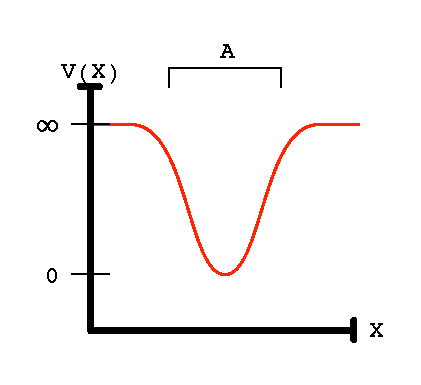
\includegraphics[scale=0.7]{figures/realWell2.eps}}
  \hspace{0.5 in}
  \subfloat[With realistic potential well]{\includegraphics[scale=0.7]{figures/realWell.eps}}
    \caption{Difference between the assumed potential well and the more ``realistic'' well}
    \label{potWells}
\end{figure}


\begin{figure}[h]
  \centering
  \subfloat[With no electric field]{\includegraphics[scale=0.7]{figures/fakeWell.eps}}
  \hspace{0.5 in}
  \subfloat[With electric field]{\includegraphics[scale=0.7]{figures/fakeFieldWell.eps}}
    \caption{How the potential well is affected by the presence of an electric field}
\end{figure}


\section{Finite Difference Method}
The finite difference method is one of several numerical methods that can be used in approximating
solutions to differential equations \cite{Hamming}. We will work through the use of the finite 
difference method and then discuss why this method was chosen over other possible alternatives. 

\subsection{Background}
The finite difference method arose due to the inherent inability of computing devices to perform
calculations using infinitesimal calculus \cite{Hamming, zhilin}. Because taking the space
between two points to its limit is impossible on a computer, estimates of the derivative must be
used. Additionally, as a continuous representation of a function is not feasible, a function is represented
by sampling values of the function at discrete points. The distance between these points will
be referred to throughout this section as $h$. 


\begin{figure}[h]
  \centering
  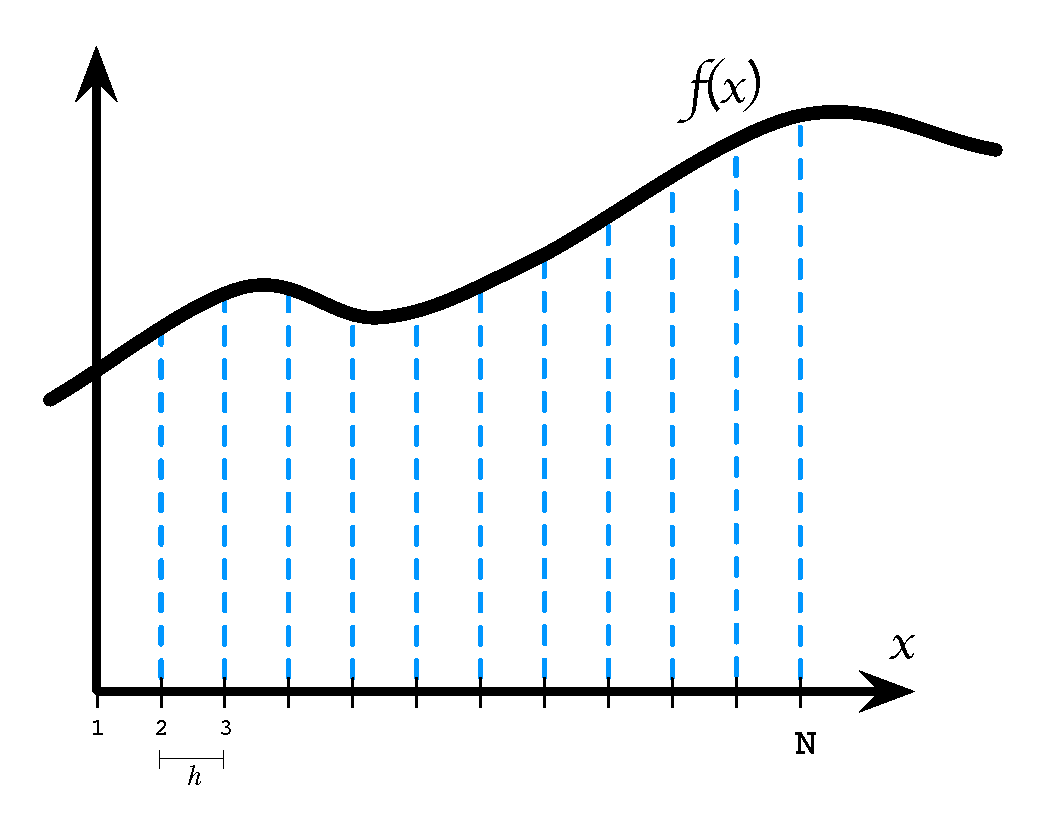
\includegraphics[scale=0.5]{figures/sampledFunc3.eps}
    \caption{Illustration of a function $f$ being sampled at discrete points}
\end{figure}

First we will define the difference operator used in FDM and then see how the difference 
operator along with the Taylor Series can be used to provide a numerical approximation of 
functions and their derivatives. 

\subsection{The Difference Operator}
A fundamental concept in the FDM is that of the difference operator. For any function 
$f$ this can be defined in three ways. As a \emph{forward difference}, a \emph{backward difference},
or as a \emph{central difference}. These are defined as follows

For the \emph{forward difference}:
\begin{equation}
\label{eq:forwardDiff}
\Delta f(x) \equiv  f(x + h) - f(x)
\end{equation}

For the \emph{backward difference}:
\begin{equation}
\label{eq:backDiff}
\nabla f(x) \equiv  f(x) - f(x - h)
\end{equation}

And for the \emph{central difference}:
\begin{equation}
\label{eq:centDiff}
\delta f(x) \equiv  f(x + \frac{1}{2}h) - f(x - \frac{1}{2}h)
\end{equation}


An important property of the difference operator that is utilized in our implementation is its linearity,
 and therefore
$$\Delta (af(x) + bg(x)) = a \Delta f(x) + b\Delta g(x) $$
where $a$ and $b$ are constants \cite{Hamming}. 

Just as with derivatives in the infinitesimal calculus, you can preform this operation repeatedly. Using the difference
operator twice, $\Delta [\Delta f(x) ] \equiv \Delta ^2 f(x) $, would correspond to the second derivative of the function. 
With the forward difference operator this is done as follows

\begin{align}
 \Delta ^2 f(x)&= \Delta [\Delta f(x)]  \nonumber\\
		&= \Delta [f(x + h) - f(x)] \nonumber\\
		&= \Delta f(x + h) - \Delta f(x) \nonumber\\  
		&= \Delta f(x + h) - (f(x + h) - f(x)) \nonumber \\
		&= f(x + 2h) - f(x + h) - (f(x + h) - f(x)) \nonumber \\ 
		&= f(x + 2h) - f(x + h) - f(x + h) + f(x) \nonumber \\
 \Delta ^2 f(x)	&= f(x + 2h) - 2f(x + h) + f(x) \label{eq:deltaSquared}
\end{align}

As we can see in equation \ref{eq:deltaSquared} the result for $\Delta ^2$ using the forward difference operator is based 
on the function's value at point $x$ and the succeeding two points $x+h$ and $x+2h$ respectively. Performing the same 
process using the central difference operator produces a slightly difference approximation

\begin{align}
 \delta ^2 f(x)&= \delta [\delta f(x)]  \nonumber\\
		&= \delta [f(x + \frac{1}{2}h) - f(x - \frac{1}{2}h)] \nonumber\\
		&= \delta f(x + \frac{1}{2}h) - \delta f(x - \frac{1}{2}h) \nonumber\\  
		&= \delta f(x + \frac{1}{2}h) - (f(x) - f(x - h)) \nonumber \\
		&= f(x + h) - f(x) - (f(x + h) - f(x)) \nonumber \\ 
		&= f(x + h) - f(x) - f(x) + f(x - h) \nonumber \\
 \delta ^2 f(x)	&= f(x + h) - 2f(x) + f(x - h)\label{eq:delta2Squared}
\end{align}


Interestingly, we can see that equations \ref{eq:deltaSquared} and \ref{eq:delta2Squared} have similar coefficients,
with each point being shifted by $-h$. Following the same steps for the backward difference would result in each point
in equation \ref{eq:deltaSquared} being shifted by $-2h$. Now that we have defined the various difference operators 
we can now apply them to approximating the derivatives of a function. 

\subsubsection{Approximating Derivatives} 
Analytically, the derivative of a function at point $x$ is the limit

\begin{equation}
  f'(x) = \lim_{h\to0} \frac{f(x + h) - f(x)}{h} \nonumber
\end{equation}

We can see that this limit looks like our forward difference operator from equation \ref{eq:forwardDiff} multiplied
by $\frac{1}{h}$. Using this form and keeping $h$ at a predetermined discrete value (not taking the limit)
is a common way of approximating the derivative \cite{Hamming, wolfram, zhilin}. Replacing the numerator with
the backward difference or the central difference provides us with approximations using those difference operators. 
Backward difference

$$f'(x) = \frac{f(x) - f(x - h)}{h} $$

Central difference

$$f'(x) = \frac{f(x + \frac{1}{2}h) - f(x - \frac{1}{2}h)}{h} $$

More generally, to approximate a function's $n^{th}$ degree derivative you must calculate the $n^{th}$ degree
difference operator and then multiply by $h^n$ \cite{Hamming, weatherley4}. For a second order derivative using
the central difference operator we are left with

\begin{equation}
f''(x) = \frac{f(x + h) - 2f(x) + f(x - h)}{h^2}
\label{eq:2ndDegreeDiffOp}
\end{equation}

The choice of which difference operator to use depends largely on the problem at hand \cite{Hamming, weatherley}. 
Some problems with specific geometric requirements may benefit from the forward or backward difference schemes \cite{weatherley}.
Weatherly uses the example of modeling advection\footnote{Advection is the transport or movement of a substance or property
(like heat or salinity) in a fluid. Convection is a subset of advection, although some use them synonymously.} as a case
where one ``must be careful to use the approximation which utilises only values that are \emph{upwind} of the point where
we wish to compute the spatial derivative'' \cite{weatherley4}. Additionally, some temporal problems may only allow
either the forward or backward difference schemes. However, in cases where a point is equally influenced
from all directions, the central difference provides more accurate solutions \cite{Hamming, weatherley, weatherley4, analysis}.
In general cases such as these, the error for the forward and backward difference schemes is $O(h)$ whereas the error 
for the central difference is $O(h^2)$ \cite{analysis, weatherley}. 
%The proofs for the error as found in \cite{weatherley} has been provided in the appendix. 

\subsection{Alternate Derivation using the Taylor Series}

Remembering the Taylor series expansion of a function

\begin{equation}
\label{eq:taylor}
f(x + h) = f(x) + f'(x)h+ \frac{f''(x)h^2}{2!} + \frac{f'''(x)h^3}{3!} + \dots + \frac{f^n(x)h^n}{n!} + R_{n}(x)
\end{equation}

Here $R_{n}(x)$ is the remainder term, which denotes the difference between the Taylor polynomial to the $n^{th}$ degree
and the actual function \cite{analysis}. 
We can `stop' the expansion at the desired derivative and solve for that derivative in order to attain an approximation. 
For example stopping at $f(x + h) = f(x) + f'(x)h$ and solving for $f'(x)$ presents us with

\begin{equation}
f'(x) = \frac{f(x + h) - f(x)}{h} - \frac{R_{1}(x)}{h}
\label{eq:taylorForward}
\end{equation}

Since our purpose is to approximate the derivative without having the actual analytic value our approximation looks like

\begin{equation}
f'(x) \approx \frac{f(x + h) - f(x)}{h}
\label{eq:taylorForwardApprox}
\end{equation}

This 1\textsuperscript{st} order approximation only uses one point to approximate the derivative. It is possible to use more 
points in the approximation by using the Taylor expansion for each desired point and then using a linear combination of these
polynomials \cite{farlow}. For example, if we required a 2\textsuperscript{nd} order approximation 
using the central difference between two point we could do this as follows

Using the Taylor expansions of two points $f(x+h)$
$$f(x+h) \approx f(x) + f'(x)h+ \frac{f''(x)h^2}{2!}$$ 

and $f(x-h)$
$$f(x-h) \approx f(x) - f'(x)h+ \frac{f''(x)h^2}{2!}$$ 

Summing these two together and solving for $f''(x)$ leaves us with

\begin{equation}
f''(x) \approx \frac{f(x + h) - 2f(x) + f(x - h)}{h^2}
\label{eq:2ndDegreeTaylor}
\end{equation}

As we can see the result is identical to the result in \ref{eq:2ndDegreeDiffOp}. Deriving the approximations through
the Taylor series allows a greater flexibility for customizing solutions to different problems as the approximation
can be derived from the specified points ($f(x+h)$ and $f(x-h)$ in our case). It allows extends to greater accuracy when
more points are included in the derivation \cite{cambridge}.  

\subsection{Use with Schr\"{o}dinger Equation}
Remembering the time-independent Schr\"{o}dinger equation
\begin{equation}
E\psi = \hat{H}\psi = -\frac{\hbar ^2}{2m}\nabla ^2\psi + V\psi \nonumber
\end{equation}

For this example we will work in only one dimension and then show how we can extend it to three dimensions. 
In one dimension this requires finding approximations to $\frac{\partial ^2 \psi}{\partial x}$. We can set our
sample space on the $x$ axis to have a length of $1$ starting from the origin. The space between samples of the 
wave function is given by

$$\Delta = \frac{L}{N - 1} $$

Where $N$ is the number of samples we would like to use. If we choose to have $11$ samples this will give us
$\Delta = .1$. This will give us a vector of $11$ of $\psi$ wave function samples arranged as follows 

$$\begin{bmatrix} 
        \psi _0  \\
        \psi _{.1}  \\
        \psi _{.2} \\
        \vdots    \\
        \psi _{1} 
   \end{bmatrix}
$$


If we remember equations \ref{eq:2ndDegreeDiffOp} and \ref{eq:2ndDegreeTaylor} we can approximate the second 
derivative of $\psi$ at these points
using the function's value at that point and the adjacent points. So for $\psi _{n}$ this would give us
$$\frac{d ^2 \psi _{n}}{dx} = \frac{\psi _{n-\Delta} - 2\psi _{n} + \psi _{n+\Delta}}{\Delta ^2} $$

%where $h \equiv \Delta$. 
Each point in our sample space has an equivalent equation. We can of course create the following matrix representation

\begin{equation}
\frac{1}{\Delta ^2}\begin{bmatrix}
                -2     &   1    &     0    &     0   & \cdots & 0 \\
                1      &  -2    &     1    &     0   & \cdots & 0 \\
                0      &   1    &    -2    &     1   & \cdots & 0 \\
                \vdots & \vdots &   \vdots & \vdots  & \ddots & \vdots \\
                0      & \cdots &    \cdots     &     0   &    1   & -2
              \end{bmatrix}\cdot \begin{bmatrix} 
                                        \psi _1  \\
                                        \psi _{2}  \\
                                        \psi _{3} \\
                                        \vdots    \\
                                        \psi _{N} 
                                   \end{bmatrix}
\end{equation}

The dimensions of the matrix correspond to the number of samples, so for N samples the resulting matrix will be
$N \times N$ in size. This matrix represents the kinetic energy portion of the Schr\"{o}dinger equation. Without
any potential the kinetic energy matrix is equivalent to the Hamiltonian operator and we now have enough information
to solve the eigenvalue problem $E\psi = \hat{H}\psi$. In order to calculate the energy of the system taking into 
account the potential $V$ we construct a diagonal $N \times N$ matrix where the values are the potential energy at each sample
point. Therefore, $V_{nn}$ will equal the potential at point $x_{n}$. This will take the following form

\begin{equation}
\begin{bmatrix}
                V(x_1) &   0     &   \cdots & \cdots &     0 \\
                0      &  V(x_2) &    0     &        &  \vdots \\
                \vdots &   0     &   \ddots &        &  \vdots \\
                \vdots &         &          & \ddots &     0 \\
                0      & \cdots  &   \cdots &   0    &   V(x_N)
              \end{bmatrix}
\end{equation}

This matrix is added to the kinetic energy matrix and then the eigenvalues are calculated. 


 
However, what happens at the edges of our specified range ($x = 0$ and $x = 1$)? Are $x = -.1$
and $x = 1.1$ required? This is where the boundary conditions come into play. Boundary conditions define the behavior
of the function at the edges of our sample space. 
In our example we will set the boundaries to $f(0) = 0$ and $f(1) = 2$. So this gives us the following system of equations

\begin{align}
\frac{-2(0)}{.1^2} + \frac{f(.1)}{.1^2} &= 0  \nonumber \\
\frac{f(0)}{.1^2} - \frac{2f(.1)}{.1^2} + \frac{f(.2)}{.1^2} &= 0 \nonumber \\
\frac{f(.1)}{.1^2} - \frac{2f(.2)}{.1^2} + \frac{f(.3)}{.1^2} &= 0\nonumber \\
\vdots \hspace{.8in} &= \, \vdots \nonumber \\
\frac{f(.8)}{.1^2} - \frac{2f(.9)}{.1^2} + \frac{f(1)}{.1^2} &= 0 \nonumber \\
\frac{f(.9)}{.1^2} - \frac{2(2)}{.1^2} &= 0 \nonumber
\end{align}

This system is equivalent to the following matrix equation



Now that we have looked that the principles of the FDM, we can now look at how to apply it to the Schro\"{o}dinger equation.

\subsection{Sources of Error}

\section{Representation of Shapes}
In reaching our goal of modeling quantum dots of various shapes, we must look into how shapes can be defined and used in 
calculations. There are several methods and techniques in the representation of three dimensional shapes on a computer. 
Computer graphics deals with the representation of shapes to a great degree, with many sophisticated techniques having been 
developed for 3D-modeling, computer aided design (CAD), and computer gaming to name a few. Our purposes may not require
many of the sophisticated techniques that others have developed as we only require sufficient information to determine if
a point is inside or outside of a given shape. 

In the first subsection we will look at some of the prevailing techniques for representing shapes on a computer. Then we will 
look at our chosen method in greater depth. 

\subsection{Possible Representations}
Researchers have developed many methods for representing shapes in computation. Generally a distinction is made between what is 
known as \emph{raster graphics} and \emph{vector graphics} \cite{bors}; for ease of understanding we will look at these two 
paradigms in two dimensions and then explain how they can expand to three. 

\subsubsection{Raster Graphics}
Raster graphics are relatively simple to understand, but can become quite complicated for certain purposes. At its most basic, 
a two dimensional raster graphic is simply a grid made up of discrete cells (also called pixels) that are individually colored.  
Each cell withing the grid has an associated value. Depending on the coloring scheme in place the value determines the 
color of the associated cell. 

\begin{figure}[h]
  \centering
  \includegraphics[scale=1.0]{figures/rasterSquare.eps}
    \caption{Raster graphic depicting an empty and a filled square}
  \label{rasterSquare}
\end{figure}

In the case of figure \ref{rasterSquare} each cell is defined by a single bit where \verb+1+ colors the cell black and
\verb+0+ colors the cell white\footnote{In many cases, such as in a monochromatic LCD screens, it would simply be 
`on' and 'off' for each pixel}. This allows the description of an image to be stored as a matrix of values in memory. 
The matrix for the image in \ref{rasterSquare} would look as follows

\begin{verbatim}
                0 0 0 0 0 0 0 0 0 0 0 0 0 0 0 0 0 0
                0 1 1 1 1 1 1 0 0 0 0 1 1 1 1 1 1 0
                0 1 0 0 0 0 1 0 0 0 0 1 1 1 1 1 1 0
                0 1 0 0 0 0 1 0 0 0 0 1 1 1 1 1 1 0
                0 1 0 0 0 0 1 0 0 0 0 1 1 1 1 1 1 0
                0 1 0 0 0 0 1 0 0 0 0 1 1 1 1 1 1 0
                0 1 1 1 1 1 1 0 0 0 0 1 1 1 1 1 1 0
                0 0 0 0 0 0 0 0 0 0 0 0 0 0 0 0 0 0
\end{verbatim}

Not surprisingly, this method is commonly referred to as a \emph{bitmap}, although this has also become a way to 
reference any raster image that has not undergone any form of compression. 
For monochromatic images this system is extremely straight-forward. Displaying the image is a matter of iterating through
the representation in memory and setting the pixels accordingly. For color images we would not be able to use bit values for
each cell and instead would need to store the appropriate convention for that particular format. A common convention is to store
eight bits for each color component; Red, Green, and Blue (RGB)\footnote{More modern representations also include and `Alpha'
component for the level of transparency.}. This gives over 16 million different possible colors. In some image processing
toolkits such as \verb+MATLAB+ store each component in a separate matrix so as to facilitate processing the individual components
separately. 

For our purposes a simple bitmap would be sufficient to represent the
\emph{in} or \emph{out} information we require for each QD. Representing a QD would be a matter of 
storing a three dimensional matrix (for the spacial dimensions) and setting the bits that are within
the Quantum Dot to \verb+1+ and leaving all the other bits at \verb+0+. This trivializes the process of 
determining when a sample point is withing the quantum dot or not as it is encoded into the definition of 
each shape. However, there are two main
issues that make raster images less suitable for our purposes. Raster images are resolution dependent. This means that
each image is specific at a specific resolution and that scaling the image to different resolutions is not possible in a 
straightforward way, usually (read almost always) resulting in loss of quality in the resolution. For example, let us
create a representation of a circle in a $10x10$ grid

\begin{figure}[h]
  \centering
  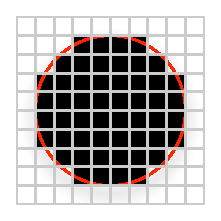
\includegraphics[scale=1.0]{figures/rasterCircle.eps}
    \caption{Circle in raster representation, with a red outline of the ``true'' circle}
  \label{rasterCircle}
\end{figure}

In \ref{rasterCircle} we have superimposed a red circle on the image to better illustrate the actual dimensions of the circle. 
Without the mathematical representation of the circle (what is in red), we would not know how to scale this image if instead of
$10x10$ we chose to use a $20x20$ grid. This is because the ``true'' shape of the circle is lost in the raster representation.  

\subsection{Geometric Primitives (Vector Graphics)}

This is where geometric primitives are useful. A geometric primitive is a `basic' building block for more complex shapes. 
Much in the same way that substances are made up of a finite number of elements, complex shapes can be constructed using
a finite set of primitives. 

An example set of primitives for two dimensions would be

\begin{itemize}
        \item lines
        \item points
        \item triangles
        \item circles
\end{itemize}

The list of primitives may seem short, but by combining these primitives in various ways we are able to define more
complex shapes. For example, two $90^{\circ}$ isosceles triangles can be placed together at their hypotenuse to form 
a square. In fact, triangles can be used to form any polygon. 

\chapter{Design and Implementation}
Now that we've looked at the necessary background information we can construct a program that will 
compute our numerical approximations. First we will look at how to represent our geometric primitives 
and how to construct the potential energy matrix from a set of shapes. We can then easily construct
the matrix for the kinetic energy. After we have looked at the basic construction of the program, we 
will look at using sparse matrix representations in order to keep the memory usage as small as possible.

\section{Potential Energy Matrix}
In this section we will focusing on the implementation of the setup of the potential energy matrix
from the Sch\"{o}dinger equation, or $V$ from $E\psi = -\frac{\hbar ^2}{2m}\nabla ^2\psi + V\psi $.

The potential energy depends on the shape of the quantum dot, and the electric field present (if any). 
%We should reference back to the diag



\section{Matlab}

\subsection{Linear Algebra in Matlab}


\subsection{Particle in a box}

\section{Matrix Representations}
\subsection{Sparse Matrix Representations}


\chapter{Results and Discussion}

\chapter{Conclusion}



\section{Further Work}

\bibliography{diss}

\end{document}
